

\tikzset{every picture/.style={line width=0.75pt}} %set default line width to 0.75pt        

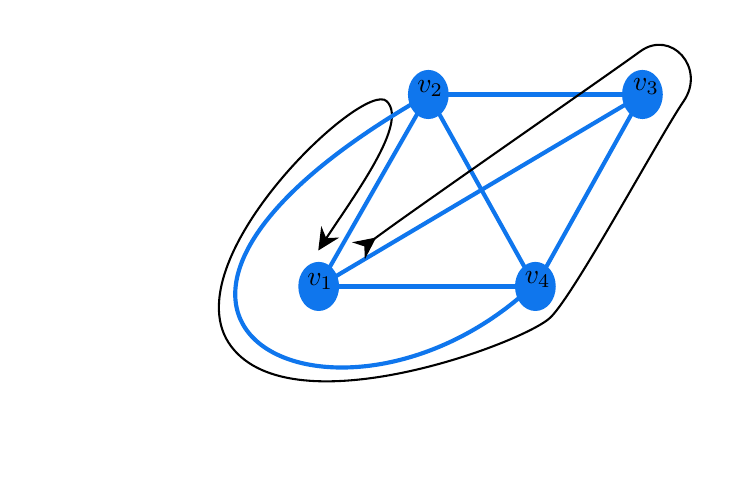
\begin{tikzpicture}[x=0.75pt,y=0.75pt,yscale=-1,xscale=1]
%uncomment if require: \path (0,191); %set diagram left start at 0, and has height of 191

%Shape: Ellipse [id:dp34898321558853973] 
\draw  [draw opacity=0][fill={rgb, 255:red, 15; green, 118; blue, 237 }  ,fill opacity=1 ] (216.97,34.83) .. controls (216.97,28.3) and (221.37,23) .. (226.79,23) .. controls (232.22,23) and (236.61,28.3) .. (236.61,34.83) .. controls (236.61,41.37) and (232.22,46.67) .. (226.79,46.67) .. controls (221.37,46.67) and (216.97,41.37) .. (216.97,34.83) -- cycle ;
%Shape: Ellipse [id:dp8581997419007412] 
\draw  [draw opacity=0][fill={rgb, 255:red, 15; green, 118; blue, 237 }  ,fill opacity=1 ] (165.4,127.32) .. controls (165.4,120.78) and (169.8,115.49) .. (175.22,115.49) .. controls (180.64,115.49) and (185.04,120.78) .. (185.04,127.32) .. controls (185.04,133.86) and (180.64,139.15) .. (175.22,139.15) .. controls (169.8,139.15) and (165.4,133.86) .. (165.4,127.32) -- cycle ;
%Shape: Ellipse [id:dp41884719294805106] 
\draw  [draw opacity=0][fill={rgb, 255:red, 15; green, 118; blue, 237 }  ,fill opacity=1 ] (61,127.32) .. controls (61,120.78) and (65.4,115.49) .. (70.82,115.49) .. controls (76.24,115.49) and (80.64,120.78) .. (80.64,127.32) .. controls (80.64,133.86) and (76.24,139.15) .. (70.82,139.15) .. controls (65.4,139.15) and (61,133.86) .. (61,127.32) -- cycle ;
%Shape: Ellipse [id:dp30805206221575077] 
\draw  [draw opacity=0][fill={rgb, 255:red, 15; green, 118; blue, 237 }  ,fill opacity=1 ] (113.83,34.83) .. controls (113.83,28.3) and (118.23,23) .. (123.65,23) .. controls (129.07,23) and (133.47,28.3) .. (133.47,34.83) .. controls (133.47,41.37) and (129.07,46.67) .. (123.65,46.67) .. controls (118.23,46.67) and (113.83,41.37) .. (113.83,34.83) -- cycle ;
%Straight Lines [id:da3826380092967572] 
\draw [color={rgb, 255:red, 15; green, 118; blue, 237 }  ,draw opacity=1 ][line width=1.5]    (175.22,127.32) -- (70.82,127.32) ;
%Straight Lines [id:da4106819955823968] 
\draw [color={rgb, 255:red, 15; green, 118; blue, 237 }  ,draw opacity=1 ][line width=1.5]    (175.22,127.32) -- (123.65,34.83) ;
%Straight Lines [id:da7580501785731988] 
\draw [color={rgb, 255:red, 15; green, 118; blue, 237 }  ,draw opacity=1 ][line width=1.5]    (175.22,127.32) -- (226.79,34.83) ;
%Straight Lines [id:da969517746532589] 
\draw [color={rgb, 255:red, 15; green, 118; blue, 237 }  ,draw opacity=1 ][line width=1.5]    (70.82,127.32) -- (226.79,34.83) ;
%Straight Lines [id:da6582184521191663] 
\draw [color={rgb, 255:red, 15; green, 118; blue, 237 }  ,draw opacity=1 ][line width=1.5]    (70.82,127.32) -- (123.65,34.83) ;
%Straight Lines [id:da21183924681168675] 
\draw [color={rgb, 255:red, 15; green, 118; blue, 237 }  ,draw opacity=1 ][line width=1.5]    (226.79,34.83) -- (123.65,34.83) ;
%Curve Lines [id:da3222564220290218] 
\draw [line width=0.75]    (97.54,104.46) .. controls (118.51,88.9) and (210.84,24.98) .. (225.61,14.15) .. controls (240.61,3.15) and (257.61,22.15) .. (246.61,38.15) .. controls (235.61,54.15) and (194.61,130.15) .. (182.61,142.15) .. controls (170.61,154.15) and (58.61,196.15) .. (28.61,156.15) .. controls (-1.39,116.15) and (92.61,27.16) .. (103.61,38.09) .. controls (114.28,48.7) and (88.26,82.89) .. (72.08,107.75) ;
\draw [shift={(70.61,110.03)}, rotate = 302.62] [fill={rgb, 255:red, 0; green, 0; blue, 0 }  ][line width=0.08]  [draw opacity=0] (10.72,-5.15) -- (0,0) -- (10.72,5.15) -- (7.12,0) -- cycle    ;
\draw [shift={(98.52,103.74)}, rotate = 503.13] [fill={rgb, 255:red, 0; green, 0; blue, 0 }  ][line width=0.08]  [draw opacity=0] (10.72,-5.15) -- (0,0) -- (10.72,5.15) -- (7.12,0) -- cycle    ;
%Curve Lines [id:da7766481202964295] 
\draw [color={rgb, 255:red, 15; green, 118; blue, 237 }  ,draw opacity=1 ][line width=1.5]    (123.65,34.83) .. controls (-68.39,144.15) and (81.61,215.15) .. (175,126) ;

% Text Node
\draw (63.82,119.72) node [anchor=north west][inner sep=0.75pt]    {$v_{1}$};
% Text Node
\draw (116.82,26.72) node [anchor=north west][inner sep=0.75pt]    {$v_{2}$};
% Text Node
\draw (220.82,25.72) node [anchor=north west][inner sep=0.75pt]    {$v_{3}$};
% Text Node
\draw (168.61,118.55) node [anchor=north west][inner sep=0.75pt]    {$v_{4}$};


\end{tikzpicture}